\documentclass[ncrna,article,submit,moreauthors,pdftex,10pt,a4paper]{mdpi} 
\usepackage{color}
\usepackage{subfigure}
\newcommand{\TODO}[1]{\begingroup\color{red}#1\endgroup}
\newcommand{\update}[1]{\begingroup\color{blue}#1\endgroup}
%=================================================================
\firstpage{1} 
\makeatletter 
\setcounter{page}{\@firstpage} 
\makeatother 
\articlenumber{x}
\doinum{10.3390/------}
\pubvolume{xx}
\pubyear{2016}
\copyrightyear{2016}
\externaleditor{Academic Editor: name}
\history{Received: date; Accepted: date; Published: date}
\history{ }
%=================================================================
\Title{Rare Splice Variants in Long Non-Coding RNAs}

\Author{Rituparno Sen$^{1}$, Gero Doose$^{2}$, 
   Peter F. Stadler$^{2-8}$*}

% Authors, for metadata in PDF
\AuthorNames{Rituparno Sen, Gero Doose, Peter F. Stadler}

\address{%
  $^{1}$Bioinformatics Group, Dept.\ Computer Science, and
  Interdisciplinary Center for Bioinformatics, University Leipzig,
  H{\"a}rtelstrasse 16-18, D-04107 Leipzig, Germany\\
  $^{2}$ecSeq Bioinformatics, Brandvorwerkstra{\ss}e 43,
  D-04275 Leipzig, Germany\\
  $^{3}$German Centre for Integrative Biodiversity Research (iDiv)
  Halle-Jena-Leipzig, Competence Center for Scalable Data Services and
  Solutions; Leipzig Research Center for Civilization Diseases; and Leipzig
  Research Center for Civilization Diseases (LIFE), University Leipzig\\
  $^{4}$Max Planck Institute for Mathematics in the Sciences,
  Inselstra{\ss}e 22, D-04103 Leipzig, Germany\\
  $^{5}$Fraunhofer Institute for Cell Therapy and Immunology,
  Perlickstrasse 1, D-04103 Leipzig, Germany\\
  $^{6}$Center for RNA in Technology and Health, Univ. Copenhagen,
  Gr{\o}nneg{\aa}rdsvej 3, Frederiksberg C, Denmark\\
  $^{7}$Santa Fe Institute, 1399 Hyde Park Road, Santa Fe NM 87501, USA }

\corres{Correspondence: studla@bioinf.uni-leipzig.de; Tel.: +49 341 97-16690}

\abstract{\TODO{rewrite!} Long noncoding RNAs (lncRNAs) are constantly being discovered and
  we are in a nascent stage of understanding their sequence structure. We
  performed statistical analyses on exon and intron content of lncRNA
  annotation data from different publicly available annotation datasets.
  We have used sophisticated alignment algorithms as well as custom
  analysis scripts to investigate the transcriptomic structure of lncRNAs.}

\keyword{lncRNA, splice junctions, GENCODE, lncRNA isoforms}

\begin{document}

\section{Introduction}

Long non-coding RNAs (lncRNAs) are an important part of the mammalian
transcriptome \cite{Clark:11a,ENCODE:12}. Although the set of lncRNAs that
is well understood with respect to biological function and molecular
mechanism is still limited, it is rapidly expanding. Genes such as ANRIL
\cite{Li:16A,Aguilo:16}, HULC \cite{Yu:17}, MALAT1 \cite{Liu:17}, TUG1
\cite{Li:16}, or Xist \cite{daRocha:17} may serve as examples. Wide-spread
roles include, but are not limited to, interactions with chromatin to
silence or activate chromatin \cite{guttmannat2012,Deng:16} and the
regulation of splicing \cite{Luco:16}. Still the coverage and precision of
the lncRNA annotation lack behind the accurate maps of protein-coding
genes.  The GENCODE project \cite{harrow2012} provides the most accurate
transcript and gene annotation for the human genome. It is a combination of
manual and automated annotation techniques which endeavours to list gene
features from HAVANA and Ensembl datasets. Detailed surveys of expression
patterns across many tissue and cell-types, see e.g.\
\cite{cabili2011,MasPonte:17,Hon:17} provide evidence for intricate
regulatory networks in which lncRNAs are key players.

There is mounting evidence, however, that lncRNA isoforms may differ
drastically in their biological function \cite{Holdt:13a,Bozgeyik:16}. Due
to their usually low expression values, gene models for lncRNAs
historically were often truncated, a situation that only has been improving
recently.  Notably, the recent lncRNA atlas by Hon \emph{et al.}
\cite{Hon:17} specifically aimed at providing accurate 5' ends. The
situation is still more difficult at the 3' side, since long, large
unspliced 3' regions make it difficult determine complete transcript from
Illumina data, see e.g.\ \cite{Mercer:10,Engelhardt:15a}. Furthermore,
lncRNAs such as ANRIL \cite{Holdt:13a}, exhibit complex patterns of
alternative splicing. Even in extremely well-studied protein-coding loci,
rare isoforms keep being discovered \cite{Hoffmann:14a}. It thus remains an
unresolved question to what extent the current maps of lncRNAs are complete
both in terms of the number of expressed loci/gene and in terms of the
variability of their isoforms.

One component towards answering this question is to ask to what extent the
transcript portfolio of a particular cell type has been mapped completely.
Conversely, one asks in this context to what extent reported transcripts
are noise. To address these issues we investigate here a very large set of
transcriptome data from B cell lymphomas. By virtue of aggregating hundreds
of independently generated transcriptome data set we can study in detail if
and the set of detectable splice junctions converges to a consensus.

\section{Results}

To better understand the distribution and structure of rare isoforms in the
the human transcriptome we investigated systematically the influence of the
dataset size on the complexity of inferred gene structures. We focussed on
RNA-Seq data from 111 lymphoma samples consisting of the different subtypes
BL, FL and DLBCL that was published in the context of the ICGC MMML-Seq
project \cite{Richter:12a}. The RNA-Seq data comprised of a total of more
than 10 billion mapped reads. Using GENCODE version 19 as reference, we
obtained set of 5,257 lncRNAs that were detectably expressed in our
lymphoma data.

Fig.~\ref{fig:saturation} summarize the effect of increasing coverage on
the estimated average number of introns per gene locus. Here, only the
subset of expressed lncRNAs with at least one annotated intron is used to
reduce the chance of erroneously or ambigously mapped reads. The data
qualitatively reproduce that observation of the ENCODE project that there
is a large difference in the average number of splice junctions between
protein-coding loci and ncRNAs \cite{Derrien:12}. Although restricted to a
quite narrowly defined cancer type, the average number of introns in
lncRNAs is larger by about one that the GENCODE data set, which uses a
composite of a broad range of cell lines and tissues. This clearly is an
effect of the exteme sequencing depth of combined lymphome data. 

\begin{figure}[t]
\begin{center}
  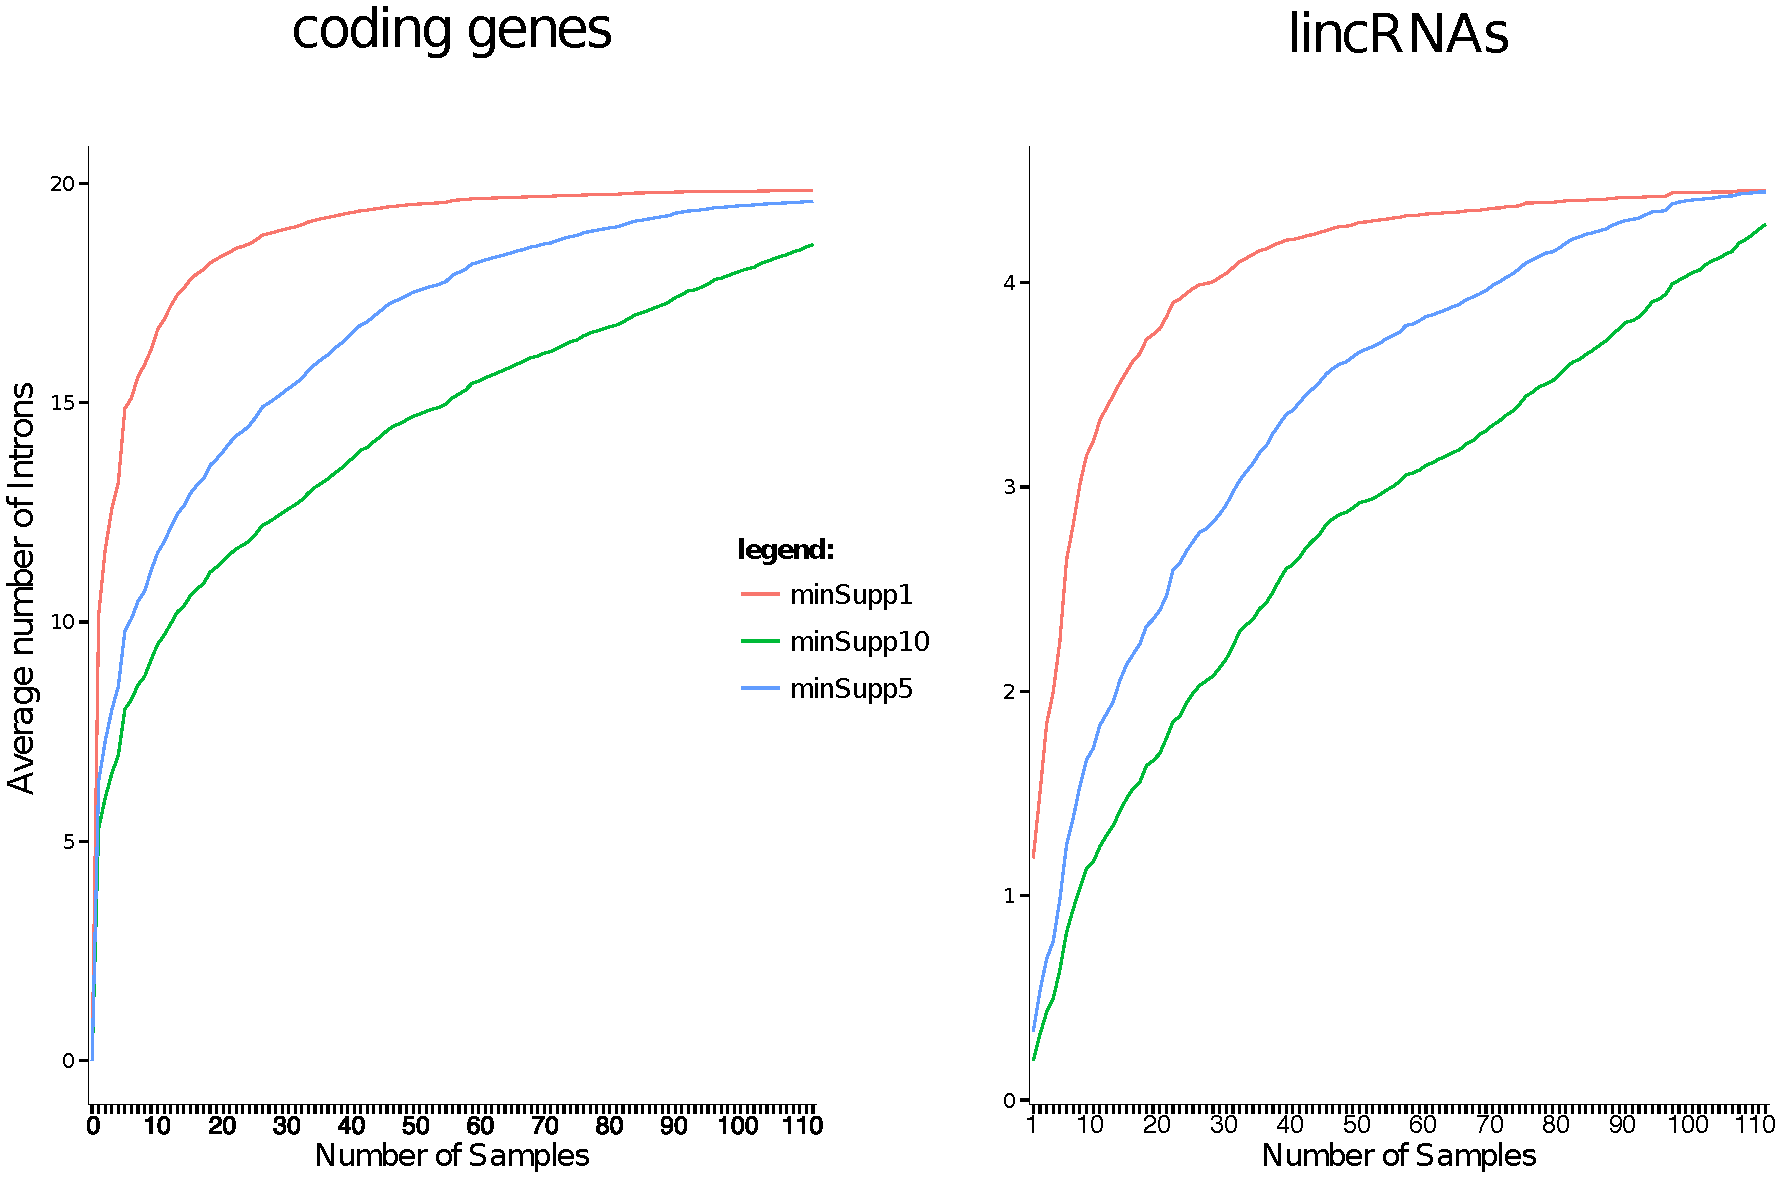
\includegraphics[width=0.8\textwidth]{saturation}
\end{center}
\caption{Saturation curves for the number introns as a function of the 
  number of independent transcriptome samples. The lncRNAs data refer to 
  annotated 1,441 genes in the lymphome data set with a least one intron. 
  }
  \label{fig:saturation} 
\end{figure}

The curves also show that data saturate very slowly, requiring dozens or
even a hundred samples to reach the plateau value. The data shows that the
detected splice junctions are unlikely to be noise: nearly all junctions
seen in at least one sample are reproduced also in 5, and most of them can
be seen in 10 samples, attesting their physical reality. 

In Fig.~\ref{fig:compare} we compare the data in more detail with the
GENCODE v.19 annotation. For the case of protein-coding loci we tend to
miss some splice junctions at loci that are extremely lowly expressed in
the lymphome transcriptomes. This is not surprising, as rare variants of
course are easier to detect in transcriptomes where they are more highly
expressed; after all, the GENCODE annotation is a composite of vastly
diverse cell types and tissues. It is interesting to note, however, that we
systematically observe more introns at moderate RPKM values even from the
very narrowly defined cell types used here. This attests that large numbers
of well-defined but rare isoforms so far have eluded annotation.

\begin{figure}[ht]
  \begin{center}
    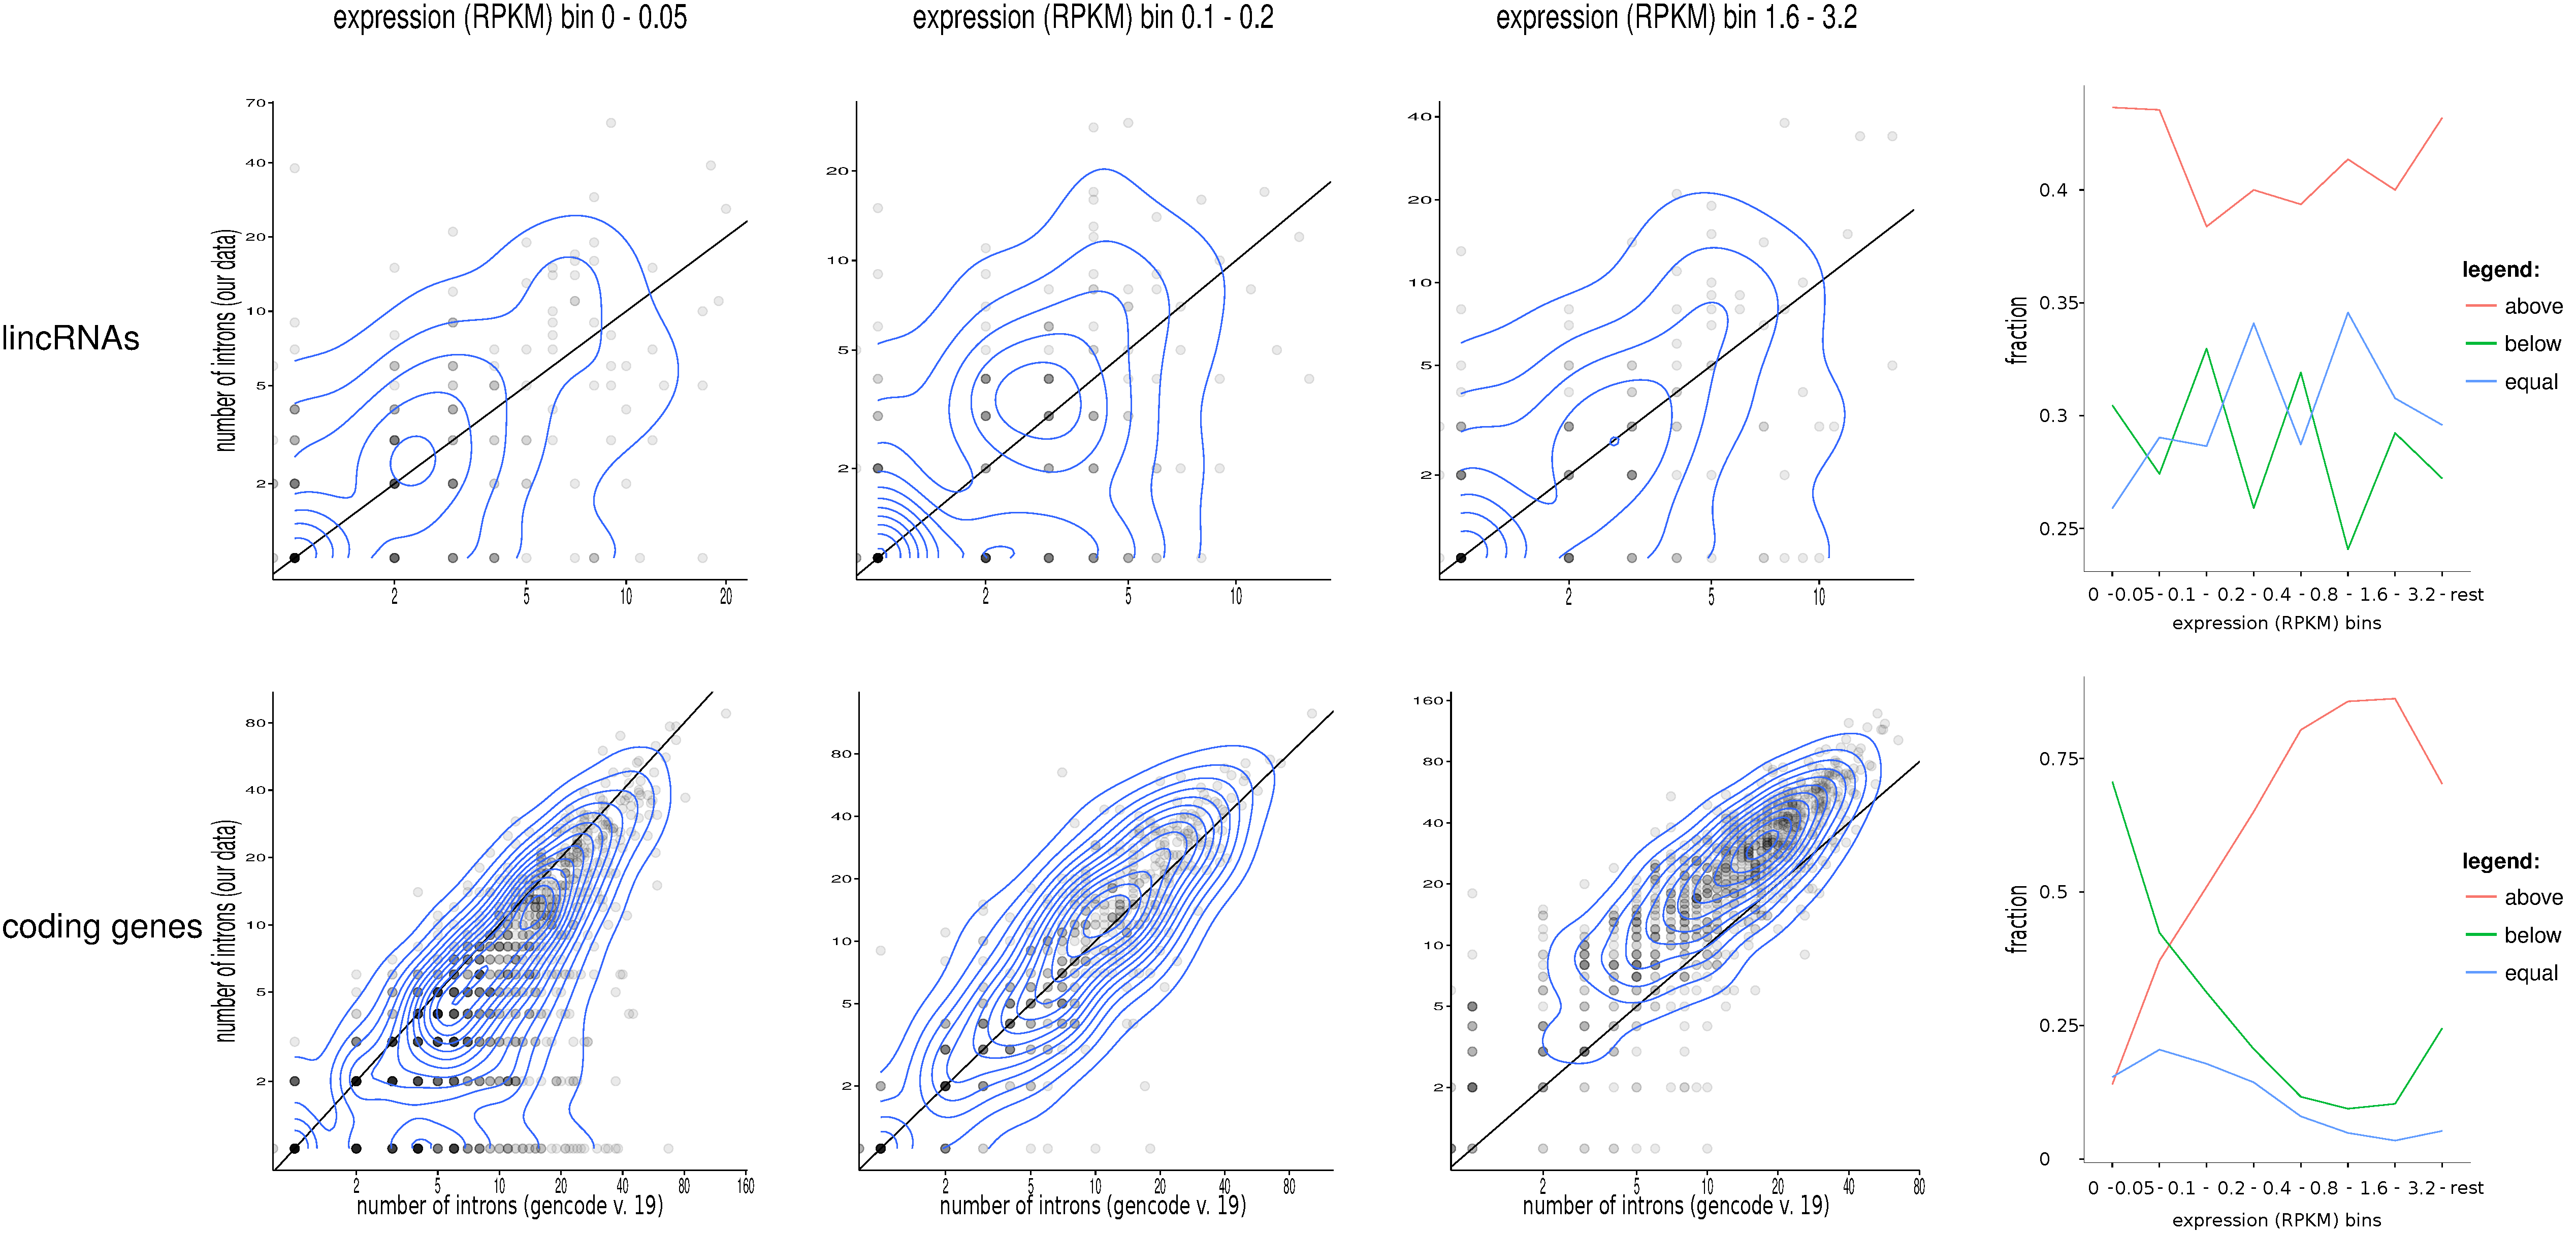
\includegraphics[width=\textwidth]{Fig1}
  \end{center}
  \caption{Scatterplots for different number of expression bins for
    lincRNAs and coding genes.  The diagonal, where $x=y$ is marked by a
    line. Points above the line are those genes for that we calculate more
    introns compared to GENCODE v.19.  The right-most column shows the
    fraction of genes for which show more (red), the same (blue), or fewer
    (green) distinct splice junctions in the lymphoma data compared to
    GENCODE v.19.  For the coding genes there is clear dependence of these
    fractions on the expression level: for highly expressed mRNAs, we
    systematically predict more (rare) splice variants. For mRNAs that are
    very lowly expressed in the lymphoma data set, GENCODE v.19 has more
    complex gene models. In contrast, we systematically see more introns in
    lncRNAs that annotated by GENCODE.}
  \label{fig:compare}
\end{figure}

Comparing to existing annotation we find that lncRNAs exhibit
systematically larger numbers of exons and introns compared to GENCODE. The
discrepancy is moderate, however, and pertains in particular to lncRNAs
that already have a large number of exons annotated.  Around 41\% of genes
are found to have more number of introns. 14\% of the genes have at least
one intron more and 19\% have more than two introns.

In Fig.~\ref{fig:examples} we show two examples that appear substantially
more complicated in our data in the GENCODE annotation. No functional
annotation is available at present for either locus. As the figure shows,
at least some of the additional exons also appear in EST data tracks
provided by the UCSC genome browser.

\begin{figure}[t]
\begin{center}
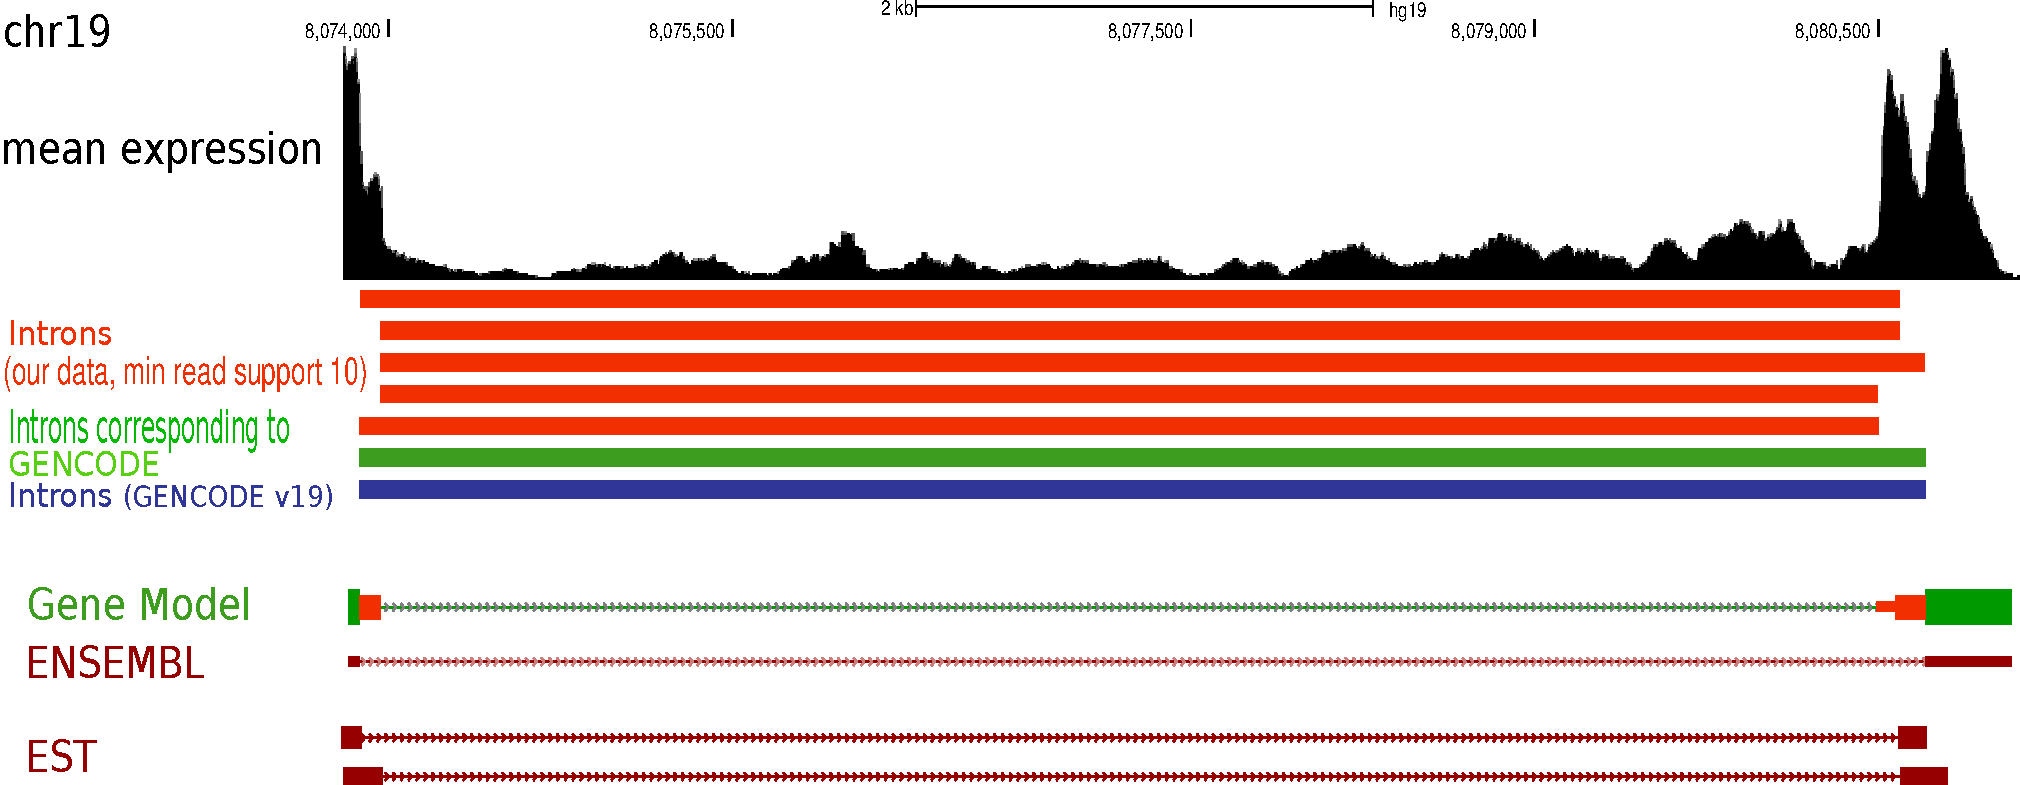
\includegraphics[width=\textwidth]{267939.pdf}\\[1em]
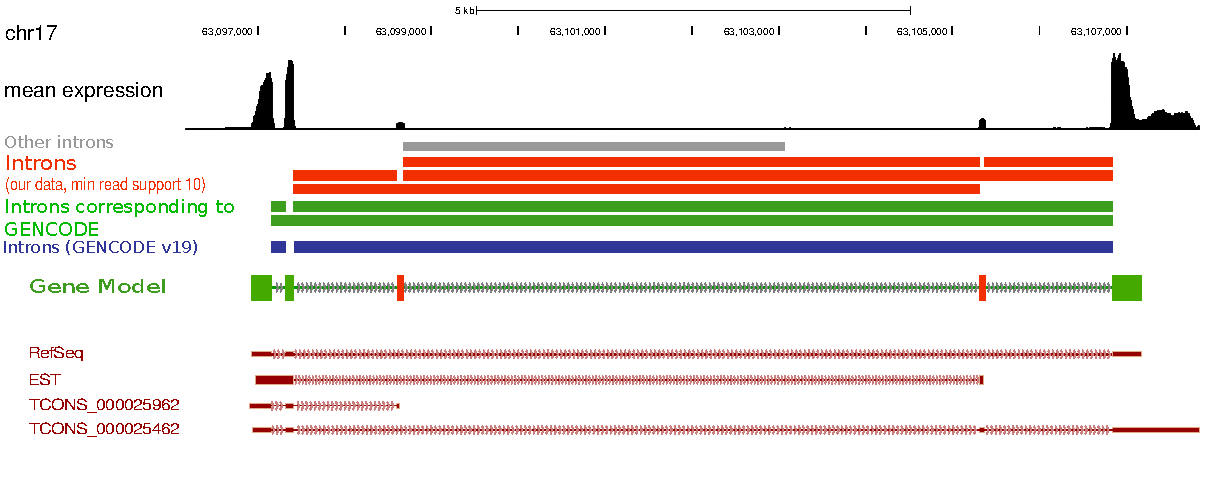
\includegraphics[width=\textwidth]{example.pdf}
\end{center}
\caption{Two examples with previously unannotated splice junctions and
  introns.  (top) In ENSG00000267939 we find 6 introns and two additional
  exons compared to a single intron described in GENCODE v19.  (below) For
  ENSG00000263470 we find 8 introns plus a likely false positive compared
  to 2 introns in GENCODE.}
\label{fig:examples} 
\end{figure}

\section{Concluding Remarks} 

We have shown that human transcriptome data harbour a large number of rare
exons (and thus also introns) that have remained unannotated. Due to their
low abundance, they appear only when data from large scale experiments are
pooled. As shown in Figure~\ref{fig:saturation} they nevertheless can be
reproduced very accurately. There is very little noise in these data, as
shown by the near perfect saturation of the average number of splice
junctions per gene. Transcriptional noise, whether biological or technical
would result in a linear increase of the number of detected junctions as
function of the size of the data set. If such a slope exists it is too
small to be detectable from our data. 

\TODO{salbungsvolle schlusssaetze} 
We can see that the annotation of lncRNAs is a very difficult task. The annotation databases cannot completely encompass the entire transcriptome accurately. Alternative splicing plays a substantial role in it. The low availability of splicing machinery related data also contributes to the cause of low number of annotated rare isoforms. Advances in technology and further research would definitely broaden our vision in the future.

\section{Materials and Methods}

The 111 RNA-seq lymphoma samples from the ICGC MMML-Seq project
\cite{Richter:12a} were mapped onto the human reference genome hg19 using
the splicing-aware mapping tool \textit{segemehl}, version $0.1.7$
\cite{Hoffmann:09a,Hoffmann:14a} with split-read mapping (option
\texttt{-S}) enabled in addition to the default parameters. The total
number of reads were around 120 million per sample. The read length was 101
and around 90\% of the reads were mappable.

Then read support for all identified splice junctions, i.e., genomic
intervals spanning exon-exon boundaries, were calculated. Since
\textit{segemehl} identifies split-reads independently of any annotation,
we consider all splice junctions located within genomic coordinates taken
from GENCODE version 19 as potential introns belonging to that GENCODE
gene. In order to call an intron, we require at minimum of $1$, $5$, or
$10$ reads representing the junction.  This procedure was performed using
the complete range of all dataset sizes from one sample to all 111 samples.
Normalized mean expression values, quantified as RPKM (reads per kilobase
and million reads) were averaged over all 111 samples and used to define a
gene's expression level in the lymphoma data set in Fig.\
\ref{fig:compare}. We only considered genes with that were supported by at
least 10 reads in our analysis.

To analyse the annotation landscape of lncRNAs, we used the whole
transcriptome sequencing data from GENCODE (versions 7 through 24)
\cite{harrow2012}, Ensembl (release 54 and 83) \cite{flicek2014}, NONCODE
(version of 2016) \cite{zhao2016}, and the dataset by Cabili \textit{et
  al.}  \cite{cabili2011}. We included the categories ``antisense'',
``lincRNA'', ``processed\_transcript'' and ``sense\_intronic biotypes'' as
lncRNAs.  The annotation data were used to define the location of
individual genes to count the total number of introns. In order to address
changes in the annotated gene structures over time we used the GENCODE v.19
genes as reference. The intersection of GENCODE v.19 with the loci that are
supported by at least 10 reads in the lymphoma data set comprises 5,257
lincRNAs.

An inhouse pipeline was used to handle the mapped data, aggregate the
multiple transcriptomes, and to compute the summary statistics of
interest. Input datasets are provided in the standard GTF format and
report, for each gene, its exact location as well as its set of constituent
transcripts. Within a gene, transcripts typically overlap and share exons.
We therefore first determined a collection of unique exons for each gene,
which was subsequently used to determine the unique introns. Mean and
median number of introns and exons per gene were computed from the number
of unique exons and introns, resp., i.e., without considering how often
they appear in distinct transcripts.

\begin{table}[ht]
  \caption{lncRNA genes catalogued by various annotation systems. The
    average number of exons and introns per transcript is given in the
    (avg.) column.} 
\label{tab:consortia}
\begin{center}\small
\begin{tabular}{|l|rr|rr|rr|}
  \hline
  & Genes & Transcripts & Exons & (avg.) & 
                        Introns & (avg.) \\ 
   \hline
  Ensembl 83   &   9597 &  14038 &  42819 & 3.05 &  28781 & 2.05 \\ 
  Ensembl 54   &  15710 &  26799 &  67583 & 2.52 &  51877 & 1.94 \\ 
  Cabili 2011  &   8263 &  14353 &  33045 & 2.30 &  18607 & 1.30 \\ 
  NONCODE 2016 & 160376 & 233696 & 536111 & 2.29 & 305771 & 1.31 \\ 
  GENCODE v7   &   9580 &  14984 &  42060 & 2.81 &  28998 & 1.94 \\ 
  GENCODE v24  &  15941 &  28031 &  68457 & 2.44 &  45016 & 1.61 \\ 
   \hline
\end{tabular}
\end{center}
\end{table}

\begin{table}[ht]
  \caption{Overlap between lncRNAs expressed in the lymphoma dataset 
    and different versions of the GENCODE annotation.} 
\label{tab:gencode}
\begin{center}\small
\begin{tabular}{|l|rr|rr|rr|}
  \hline
  & Genes & Transcripts & Exons & (avg) & Introns & (avg) \\ 
   \hline
  v7  & 3296 & 4563 & 12584 & 2.76 &  8394 & 1.84 \\
  v19 & 5257 & 7487 & 18774 & 2.51 & 12010 & 1.60 \\
  v24 & 4961 & 7318 & 18685 & 2.55 & 12202 & 1.67 \\ 
   \hline
\end{tabular}
\end{center}
\end{table}

A comparison of the published annotation data showed substantial changes in
the average number of exons per genes. Not surprisingly, the later ENSEMBL
version 83 reports on average more introns per lncRNA gene, presumably in
response to more complete gene models. It is worth noting, however, that
the number of annotated lncRNAs dropped from more than 15,000 to less than
10,000 between versions 54 and 83, suggesting that the ENSEMBL annotation
is far from complete and includes only the most stringently curated
lncRNAs. In contrast, the NONCODE database is very inclusive and provides
more than an order of magnitude more entries. An interesting trend in the
GENCODE annotation is that the number of exons per lncRNAs has been
decreasing slightly over time (Tab.~\ref{tab:consortia}).  We used the UCSC
genome browser \cite{Kent:02} to visualize additional introns.

%%%%%%%%%%%%%%%%%%%%%%%%%%%%%%%%%%%%%%%%%%
\vspace{6pt} 

%%%%%%%%%%%%%%%%%%%%%%%%%%%%%%%%%%%%%%%%%%

%%%%%%%%%%%%%%%%%%%%%%%%%%%%%%%%%%%%%%%%%%
\acknowledgments{This work was supported in part by the Deutsche
  For\-schungs\-ge\-mein\-schaft grant no.\ NO 920/6-1 as part of SPP
  1738. RS is supported by the Deutscher Akademischer Austauschdienst
  (DAAD).}

\authorcontributions{PFS designed the study, RS and GD analyzed the data,
  all authors contributed to the interpretation of the results and the
  writing of the manuscript.}

%%%%%%%%%%%%%%%%%%%%%%%%%%%%%%%%%%%%%%%%%%
\conflictofinterests{The authors declare no conflict of interest.}

%%%%%%%%%%%%%%%%%%%%%%%%%%%%%%%%%%%%%%%%%%
%% optional
\abbreviations{The following abbreviations are used in this manuscript:
\par\noindent 
\begin{tabular}{@{}ll}
lncRNA & long non-coding RNA\\
rRNA   & ribosomal RNA\\
RPKM   & reads per kilobase per million mapped reads\\
BL     & Burkitt lymphoma\\
FL     & folicular lymphoma\\
DLBCL  & diffuse large B cell lymphoma\\
\end{tabular}}

\bibliographystyle{mdpi}
\bibliography{references}
\end{document}

